\documentclass[11pt,a4paper]{article}

% -------- Packages --------
\usepackage[T1]{fontenc}
\usepackage{lmodern}
\usepackage[a4paper, top=2cm, bottom=2.2cm, left=2.3cm, right=2.3cm, footskip=1.2cm]{geometry}
\usepackage{amsmath}
\usepackage{microtype}
\usepackage{booktabs}
\usepackage{tabularx}
\usepackage[shortlabels]{enumitem}
\usepackage{array}
\usepackage[table]{xcolor}
\usepackage{titlesec}
\usepackage{fancyhdr}
\usepackage{tikz}
\usepackage{tcolorbox}
\tcbuselibrary{skins}
\usepackage[hidelinks,
  pdftitle={DATP-CP Research Dossier},
  pdfsubject={Calibration-Channel Poisoning in Federated IoT Anomaly Detection},
  pdfkeywords={federated learning, anomaly detection, calibration poisoning, N-BaIoT}
]{hyperref}

\usetikzlibrary{arrows.meta, positioning}

% -------- Colors --------
\definecolor{navyhead}{RGB}{22, 36, 72}
\definecolor{amber}{RGB}{194, 140, 45}
\definecolor{footgray}{RGB}{110, 110, 110}
\definecolor{rulegray}{RGB}{160, 160, 160}
\definecolor{boxbg}{RGB}{247, 247, 249}

% -------- Callout box styles --------
\tcbset{
  callout/.style={
    enhanced,
    left=10pt, top=5pt, bottom=5pt, right=6pt,
    boxrule=0.3pt, colframe=gray!30,
    colback=boxbg,
    borderline west={2.5pt}{0pt}{navyhead},
    arc=2pt, outer arc=2pt
  },
  ambercallout/.style={
    enhanced,
    left=10pt, top=5pt, bottom=5pt, right=6pt,
    boxrule=0.3pt, colframe=amber!40,
    colback=amber!8,
    borderline west={2.5pt}{0pt}{amber},
    arc=2pt, outer arc=2pt
  }
}

% -------- Section formatting --------
\titleformat{\section}
  {\large\bfseries\color{navyhead}}{}{0em}{}
  [\vspace{0.15em}{\color{rulegray}\hrule height 0.45pt}\vspace{0.2em}]
\titlespacing{\section}{0pt}{1.5ex plus 0.4ex minus 0.2ex}{0.5ex plus 0.2ex}

\titleformat{\subsection}
  {\normalsize\bfseries\color{navyhead}}{}{0em}{}
\titlespacing{\subsection}{0pt}{0.9ex plus 0.2ex minus 0.1ex}{0.3ex plus 0.1ex}

% -------- Lists --------
\setlist{nosep, topsep=3pt, itemsep=2pt, parsep=0pt, leftmargin=1.5em}
\setlist[enumerate]{leftmargin=1.6em}

% -------- Header / Footer --------
\pagestyle{fancy}
\fancyhf{}
\renewcommand{\headrulewidth}{0pt}
\fancyfoot[C]{\small\color{footgray}DATP-CP Research Dossier \textperiodcentered\ v1.0}
\fancyfoot[R]{\small\color{footgray}\thepage}

\fancypagestyle{plain}{%
  \fancyhf{}%
  \renewcommand{\headrulewidth}{0pt}%
  \fancyfoot[C]{\small\color{footgray}DATP-CP Research Dossier \textperiodcentered\ v1.0}%
  \fancyfoot[R]{\small\color{footgray}\thepage}%
}

% -------- Misc --------
\setlength{\parindent}{0pt}
\setlength{\parskip}{3pt plus 1pt}

% Monospace constant — \hbox prevents mid-word line breaks
\newcommand{\const}[1]{\texttt{\small\hbox{#1}}}

\begin{document}
\pagestyle{fancy}

% ================================================================
% PAGE 1 — EXECUTIVE SCOPE
% ================================================================

% ---- Title block ----
{\color{navyhead}\rule{\linewidth}{2pt}}

\begin{center}
  \vspace*{0.25em}
  {\Huge\bfseries\color{navyhead} DATP-CP}\\[0.4em]
  {\Large\bfseries\color{navyhead} Research Dossier}\\[0.6em]
  {\large Calibration-Channel Poisoning in Federated IoT Anomaly Detection}\\[0.75em]
  \small
  \begin{tabular}{@{}ll@{}}
    \textbf{Version:} & v1.0\\[2pt]
    \textbf{Status:}  & Scientific and technical scoping document
  \end{tabular}\\[0.55em]
\end{center}
{\color{navyhead}\rule{\linewidth}{1.2pt}}

\vspace{0.4em}

\begin{tcolorbox}[ambercallout]
\small\textbf{Scope:} N-BaIoT threshold-scope study.
Attack surface: benign calibration scores only.
Training data, model weights, aggregation, test scores, and labels are not modified.
\end{tcolorbox}

\vspace{0.25em}

% ---- Purpose ----
\section{Purpose}

\begin{itemize}
  \item Study the post-training threshold-calibration stage as an attack surface.
  \item Modify only benign calibration scores.
  \item Preserve training data, aggregation, model weights, test scores, and test labels.
  \item Compare \const{GLOBAL\_THRESHOLD}, \const{LOCAL\_THRESHOLD}, and
    \const{CLUSTER\_THRESHOLD}.
  \item Keep claims bounded to the tested N-BaIoT protocol.
\end{itemize}

% ---- Minimal pipeline ----
\section{Minimal Pipeline}

\begin{center}
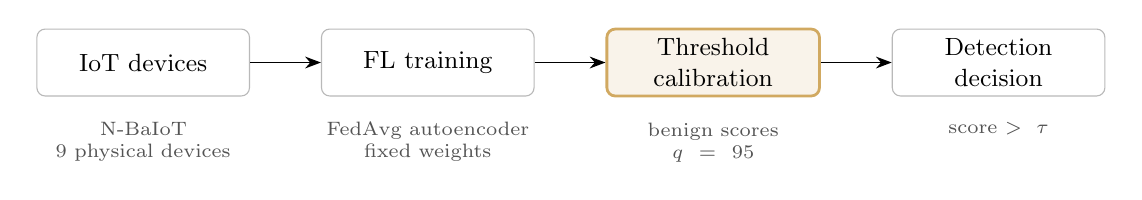
\begin{tikzpicture}[
  node distance=0.9cm,
  >=Stealth,
  box/.style={
    rectangle, draw=gray!55, fill=white,
    rounded corners=3pt,
    minimum width=2.7cm, minimum height=0.85cm,
    text centered, font=\small, align=center
  },
  amberbox/.style={
    rectangle, draw=amber!75, fill=amber!10,
    rounded corners=3pt,
    minimum width=2.7cm, minimum height=0.85cm,
    text centered, font=\small, align=center,
    line width=1pt
  },
  lbl/.style={font=\scriptsize, text width=2.7cm, align=center, text=gray!65!black}
]
  \node[box] (iot)  {IoT devices};
  \node[box,  right=0.9cm of iot] (fl)  {FL training};
  \node[amberbox, right=0.9cm of fl]  (cal) {Threshold\\calibration};
  \node[box,  right=0.9cm of cal] (det) {Detection\\decision};

  \draw[->, line width=0.6pt] (iot) -- (fl);
  \draw[->, line width=0.6pt] (fl)  -- (cal);
  \draw[->, line width=0.6pt] (cal) -- (det);

  \node[lbl, below=0.2cm of iot] {N-BaIoT\\9 physical devices};
  \node[lbl, below=0.2cm of fl]  {FedAvg autoencoder\\fixed weights};
  \node[lbl, below=0.2cm of cal] {benign scores\\$q = 95$};
  \node[lbl, below=0.2cm of det] {score $> \tau$};
\end{tikzpicture}
\end{center}

\vspace{0.1em}
{\footnotesize\itshape
Only the \textcolor{amber!80!black}{threshold calibration} step is within the attack surface.}

% ---- Scope boundary ----
\section{Scope Boundary}

\begin{tcolorbox}[callout]
\begin{itemize}
  \item Calibration scores may change.
  \item Training data does not change.
  \item Model weights do not change.
  \item Aggregation does not change.
  \item Test scores and labels do not change.
  \item AUROC invariance is a sanity check only.
\end{itemize}
\end{tcolorbox}

\clearpage

% ================================================================
% PAGE 2 — PROJECT IDENTITY AND DOCUMENT PURPOSE
% ================================================================

\section{Project Identity}

\begin{tabularx}{\linewidth}{@{} >{\bfseries}p{4.2cm} X @{}}
\toprule
\normalfont\textbf{Field} & \textbf{Value}\\
\midrule
Project acronym     & DATP-CP\\[3pt]
Full title          & Calibration-Channel Poisoning in Federated IoT Anomaly Detection\\[3pt]
Document type       & Research Dossier\\[3pt]
Version             & v1.0\\[3pt]
Status              & Scientific and technical scoping document\\[3pt]
Thesis line         & Collaborative Malware Detection with Federated Learning in IoT Networks\\[3pt]
Research branch     & Security / calibration-channel poisoning\\[3pt]
Main dataset        & N-BaIoT\\[3pt]
Client definition   & Physical IoT device as FL client\\[3pt]
Model setting       & Fixed FedAvg autoencoder\\[3pt]
Threshold policies  & \const{GLOBAL\_THRESHOLD}, \const{LOCAL\_THRESHOLD},
                      \const{CLUSTER\_THRESHOLD}\\[3pt]
Main claim scope    & Single-client calibration compromise\\
\bottomrule
\end{tabularx}

\vspace{0.6em}

\section{Document Purpose}

\subsection*{This document:}

\begin{itemize}
  \item Defines research scope.
  \item Defines scientific objectives.
  \item Defines methodological boundaries.
  \item Defines validation criteria.
  \item Defines expected deliverables.
  \item Defines risks and limitations.
\end{itemize}

\subsection*{This document is not:}

\begin{itemize}
  \item A paper draft.
  \item A presentation deck.
  \item An implementation log.
\end{itemize}

\clearpage

% ================================================================
% PAGE 3 — CONTEXT AND POSITIONING
% ================================================================

\section{Context and Positioning}

\subsection{DATP Baseline}

\begin{itemize}
  \item DATP studied threshold calibration scope in non-IID federated IoT anomaly detection.
  \item It fixed the FedAvg autoencoder and varied only the threshold policy.
  \item It showed that threshold scope governs per-client false-alarm disparity.
  \item It established calibration as a decisive operating-point variable.
\end{itemize}

\subsection{DATP-CP Rationale}

\begin{itemize}
  \item DATP-CP asks whether the same calibration stage is vulnerable.
  \item The attack occurs after training.
  \item Existing FL defenses usually focus on training, updates, or aggregation.
  \item DATP-CP studies the post-training calibration gap under strict causal isolation.
\end{itemize}

\subsection{Three-Branch Comparison}

\vspace{0.3em}
\begin{tabularx}{\linewidth}{@{} >{\bfseries\small}p{3.2cm}
                                    >{\small}X
                                    >{\small}X
                                    >{\small}X @{}}
\toprule
\normalfont & \textbf{DATP} & \textbf{DATP-CP} & \textbf{Journal extension}\\
\midrule
Scientific role
  & Performance study
  & Security study
  & Generalization study\\[4pt]
Main question
  & Which policy minimizes FPR disparity?
  & Does calibration poisoning produce policy-dependent harm?
  & Do findings generalize?\\[4pt]
Primary variable
  & Threshold policy
  & Poison fraction $f$
  & Dataset / FL protocol\\[4pt]
Adversary
  & None
  & Single compromised client
  & None\\[4pt]
Claim boundary
  & N-BaIoT, threshold-scope study
  & N-BaIoT, single-client
  & External datasets\\
\bottomrule
\end{tabularx}
\vspace{0.3em}

\subsection{Key Distinctions}

\begin{itemize}
  \item \textbf{DATP:} performance personalization.
  \item \textbf{DATP-CP:} calibration-channel security.
  \item \textbf{Journal extension:} external validation and generalization.
\end{itemize}

\clearpage

% ================================================================
% PAGE 4 — PROBLEM, RESEARCH QUESTION, OBJECTIVES, SCOPE
% ================================================================

\section{Problem}

\begin{itemize}
  \item Thresholds are computed after training.
  \item Thresholds define the final operating point.
  \item Benign calibration scores determine~$\tau$.
  \item This stage is separate from model training and aggregation.
  \item The calibration buffer may become an overlooked attack surface.
\end{itemize}

\subsection{Central Research Question}

\begin{tcolorbox}[callout]
\itshape
Does poisoning only benign threshold-calibration scores produce material,
policy-dependent downstream harm under \const{GLOBAL\_THRESHOLD},
\const{LOCAL\_THRESHOLD}, and \const{CLUSTER\_THRESHOLD}?
\end{tcolorbox}

\section{Objectives}

\begin{minipage}[t]{0.48\linewidth}
\subsection*{Scientific objectives}
\begin{itemize}
  \item Isolate threshold calibration as an attack surface.
  \item Measure material threshold movement.
  \item Compare vulnerability across threshold policies.
  \item Separate raising and lowering failure modes.
  \item Preserve causal isolation.
\end{itemize}
\end{minipage}%
\hfill
\begin{minipage}[t]{0.48\linewidth}
\subsection*{Technical objectives}
\begin{itemize}
  \item Validate clean DATP-compatible artifacts.
  \item Implement controlled benign-score replacement.
  \item Enforce valid source-objective pairs.
  \item Run paired clean-vs-poisoned comparisons.
  \item Produce reproducible outputs.
\end{itemize}
\end{minipage}

\vspace{0.5em}

\section{Scope}

\vspace{0.2em}
\begin{tabularx}{\linewidth}{@{} >{\small}X >{\small}X @{}}
\toprule
\textbf{Included} & \textbf{Excluded}\\
\midrule
N-BaIoT main study                    & Training-data poisoning\\[2pt]
Physical device clients                & Model poisoning\\[2pt]
Fixed FedAvg autoencoder               & Aggregation poisoning\\[2pt]
Benign calibration-score poisoning     & Backdoors\\[2pt]
Score-level proxy attack               & Evasion\\[2pt]
\const{GLOBAL\_THRESHOLD}             & Privacy mechanisms\\[2pt]
\const{LOCAL\_THRESHOLD}              & Deployment benchmarking\\[2pt]
\const{CLUSTER\_THRESHOLD}            & Raw-traffic attack generation\\[2pt]
$q = 95$                               & Journal-extension datasets as main evidence\\[2pt]
Single-client main study               & Model-personalization comparators\\[2pt]
Paired clean-vs-poisoned evaluation    & Universal FL robustness claims\\[2pt]
\const{RANDOM\_BENIGN} control        & Privacy guarantee claims\\
\bottomrule
\end{tabularx}

\clearpage

% ================================================================
% PAGE 5 — METHODOLOGY AND VALIDATION
% ================================================================

\section{Methodology and Validation}

\subsection{Experimental Setup}

\textbf{Dataset} — N-BaIoT; 9 physical IoT devices; one device equals one FL client;
$n_{\text{cal}} \geq 100$.

\textbf{Model} — Federated autoencoder; FedAvg; fixed model weights; clean and poisoned
runs share the same model.

\textbf{Calibration} — Benign reconstruction scores; p95 threshold rule; $q = 95$;
policies: \const{GLOBAL}, \const{LOCAL}, \const{CLUSTER}.

\subsection{Attack Mechanism}

\begin{enumerate}
  \item Select a victim client.
  \item Choose poison fraction~$f$.
  \item Select replacement positions in the benign calibration array.
  \item Sample replacement values from the victim-local benign reservoir.
  \item Recompute thresholds.
  \item Evaluate on unchanged test scores and labels.
\end{enumerate}

\vspace{0.2em}
\begin{minipage}[t]{0.54\linewidth}
\subsection{Source Strategies}
\begin{itemize}
  \item \const{HIGH\_SCORE\_BENIGN} $\to$ \const{THRESHOLD\_RAISE}
  \item \const{LOW\_SCORE\_BENIGN} $\to$ \const{THRESHOLD\_LOWER}
  \item \const{RANDOM\_BENIGN} $\to$ negative control
\end{itemize}
\end{minipage}%
\hfill
\begin{minipage}[t]{0.42\linewidth}
\subsection{Poison Fractions}
\[f \in \{0.10,\; 0.20,\; 0.40\}\]
\end{minipage}

\vspace{0.3em}

\subsection{Validation Criteria}

\vspace{0.2em}
\begin{tabularx}{\linewidth}{@{} l l X @{}}
\toprule
\textbf{Criterion} & \textbf{Metric} & \textbf{Interpretation}\\
\midrule
Signed $\Delta\tau$            & Direction             & Attack in correct direction\\[2pt]
Material $|\Delta\tau|$        & Magnitude             & Effect exceeds materiality bound\\[2pt]
$\Delta\text{TPR}$             & Detection drop        & Under \const{THRESHOLD\_RAISE}\\[2pt]
$\Delta\text{CV}(\text{FPR})$  & Alarm dispersion      & Under \const{THRESHOLD\_LOWER}\\[2pt]
Policy differentiation         & Differential response & Policies respond differently\\[2pt]
\const{RANDOM\_BENIGN}        & Control audit         & Negative-control baseline\\[2pt]
AUROC invariance               & Sanity check          & Not a primary metric\\
\bottomrule
\end{tabularx}

\vspace{0.4em}

\subsection{Claim Gates}

\begin{enumerate}
  \item \textbf{Gate 1:} Material correctly signed $\Delta\tau$.
  \item \textbf{Gate 2:} Directional effect exceeds \const{RANDOM\_BENIGN}.
  \item \textbf{Gate 3:} Downstream harm metric moves as expected.
\end{enumerate}

\subsection{Claim Classes}

\begin{itemize}
  \item \textbf{Full vulnerability:} All gates pass.
  \item \textbf{Mechanism-only:} Threshold movement only.
  \item \textbf{Calibration instability:} Negative control also moves.
  \item \textbf{Null or conditional:} Evidence insufficient.
\end{itemize}

\clearpage

% ================================================================
% PAGE 6 — DELIVERABLES, RISKS, AND GOVERNANCE
% ================================================================

\begin{minipage}[t]{0.48\linewidth}
\section{Deliverables}
\begin{itemize}[leftmargin=0pt, itemindent=0pt, label={}]
  \item \textbf{D1} Research protocol and scope definition.
  \item \textbf{D2} Attack implementation and calibration-injection pipeline.
  \item \textbf{D3} Clean artifact validation report.
  \item \textbf{D4} Poisoning experiment outputs.
  \item \textbf{D5} Figures and result tables.
  \item \textbf{D6} Conference manuscript.
  \item \textbf{D7} Reproducibility package.
  \item \textbf{D8} Presentation dossier.
\end{itemize}
\end{minipage}%
\hfill
\begin{minipage}[t]{0.48\linewidth}
\section{Work Packages}
\begin{itemize}[leftmargin=0pt, itemindent=0pt, label={}]
  \item \textbf{WP1} Scope lock and scientific boundary audit.
  \item \textbf{WP2} Clean artifact validation.
  \item \textbf{WP3} Attack implementation and validation tests.
  \item \textbf{WP4} N-BaIoT main experiment execution.
  \item \textbf{WP5} Analysis, figures, and tables.
  \item \textbf{WP6} Manuscript preparation.
  \item \textbf{WP7} Final audit and packaging.
\end{itemize}
\end{minipage}

\vspace{0.5em}

\begin{minipage}[t]{0.48\linewidth}
\section{Risks and Limitations}
\begin{itemize}
  \item Score-level proxy limitation.
  \item N-BaIoT-only main evidence.
  \item Single-client compromise main claim.
  \item No deployment benchmark.
  \item AUROC invariance is a sanity check only.
  \item With-replacement sampling may duplicate scores.
\end{itemize}
\end{minipage}%
\hfill
\begin{minipage}[t]{0.48\linewidth}
\section{Governance}
\begin{itemize}
  \item Keep claims bounded to the tested protocol.
  \item Disclose score-level proxy limitation.
  \item Treat AUROC invariance only as a sanity check.
  \item Do not convert optional extensions into main claims.
  \item Do not claim raw-traffic exploitability.
  \item Do not claim deployment readiness.
\end{itemize}
\end{minipage}

\vspace{0.6em}

\section{Research Contribution}

\begin{tcolorbox}[callout]
DATP-CP contributes:
\begin{itemize}
  \item A bounded calibration-channel threat model.
  \item Causal isolation from training and aggregation.
  \item Policy-differentiated vulnerability evidence.
  \item A bridge between DATP and adversarial robustness.
\end{itemize}
\end{tcolorbox}


\end{document}
